\section{Results}
\label{sec:results}

We got those results.

We calculate $\mathrm{B}(\muF)$, $\deltaQCD(\muR,\muF)$ and 
$\deltaEW(\muF^0)$

\subsection{\texorpdfstring{$\boldsymbol{\gamma\gamma\gamma}$}{aaa} production}
\label{sec:results:aaa}

\begin{figure}[t!]
  \centering
  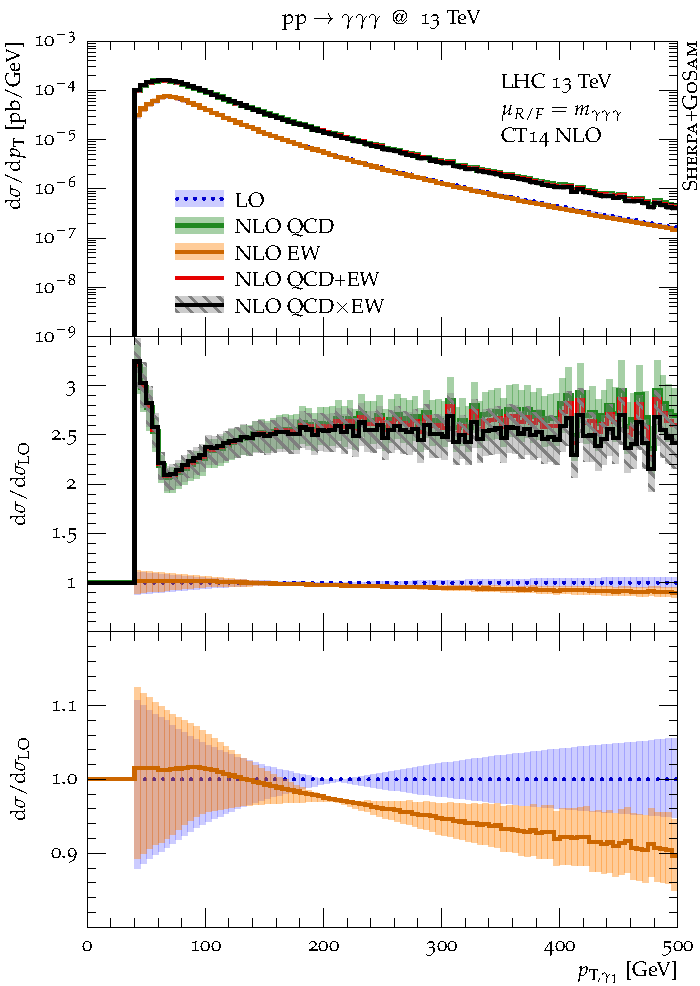
\includegraphics[width=0.32\textwidth]{figs_aaa/pT_y1}
  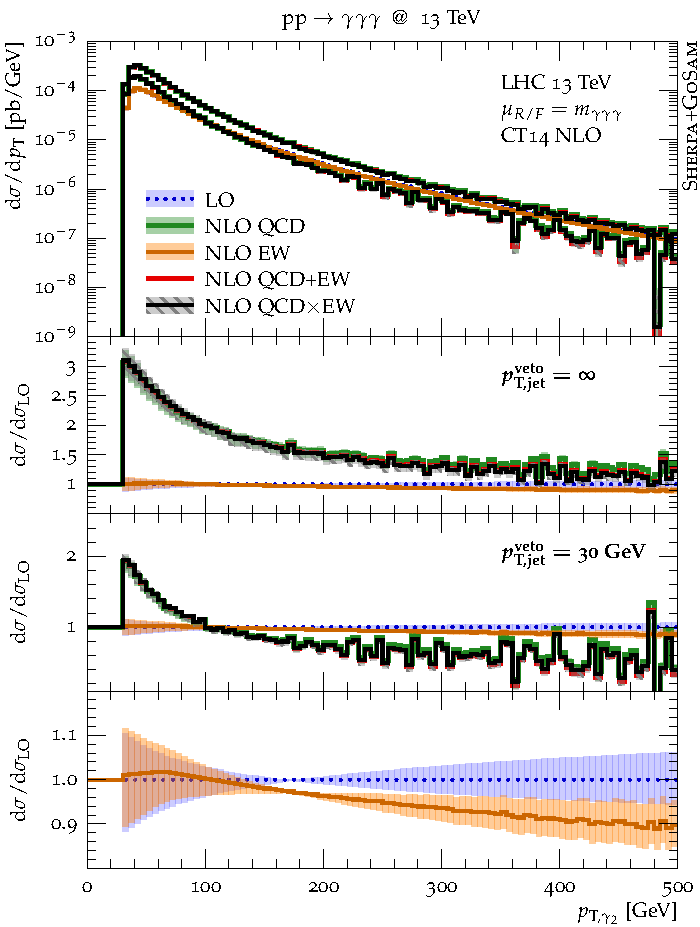
\includegraphics[width=0.32\textwidth]{figs_aaa/pT_y2}
  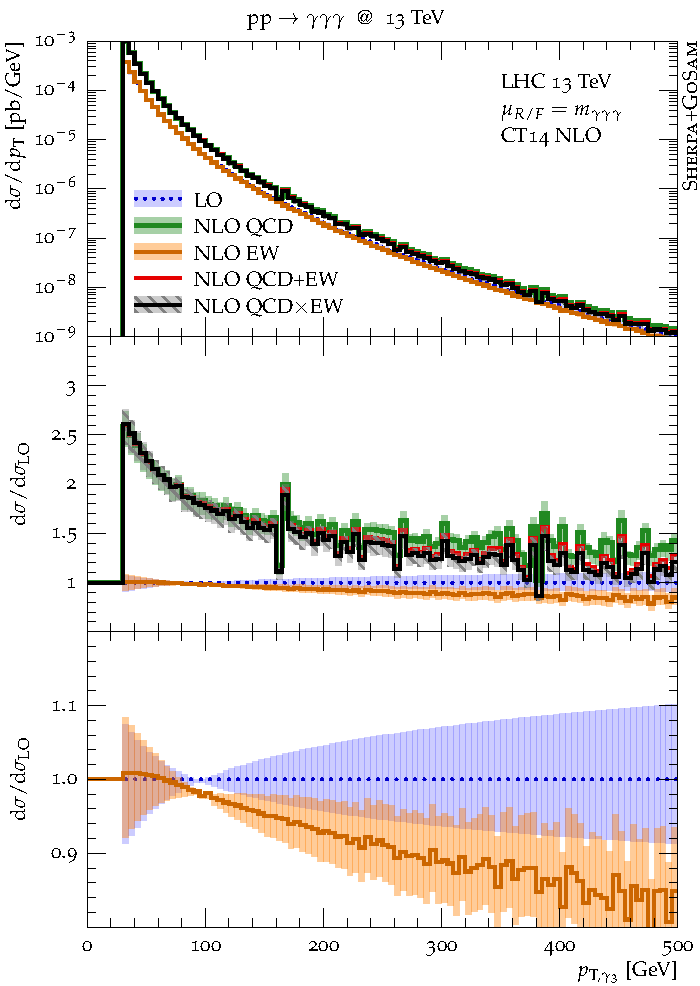
\includegraphics[width=0.32\textwidth]{figs_aaa/pT_y3}
  \caption{
    Transverse momentum of the leading (left), subleading (centre) 
    and third leading (right) photon 
    in triple photon production at the LHC at 13\,TeV. 
    The distributions are shown at LO (blue), NLO QCD (green), 
    NLO EW (orange), NLO \QCDpEW\ (red) and NLO \QCDtEW\ (black) 
    including scale uncertainties. The top ratio plot details 
    the relative corrections to the leading order cross section 
    without applying any jet veto, while the centre ratio plot 
    applies a jet veto of $p_\mathrm{T,jet}^\mathrm{veto}=\text{30\,GeV}$. 
    The lower ratio highlights the size of the electroweak corrections.
    \label{fig:aaa:pt}
  }
\end{figure}

\begin{figure}[t!]
  \centering
  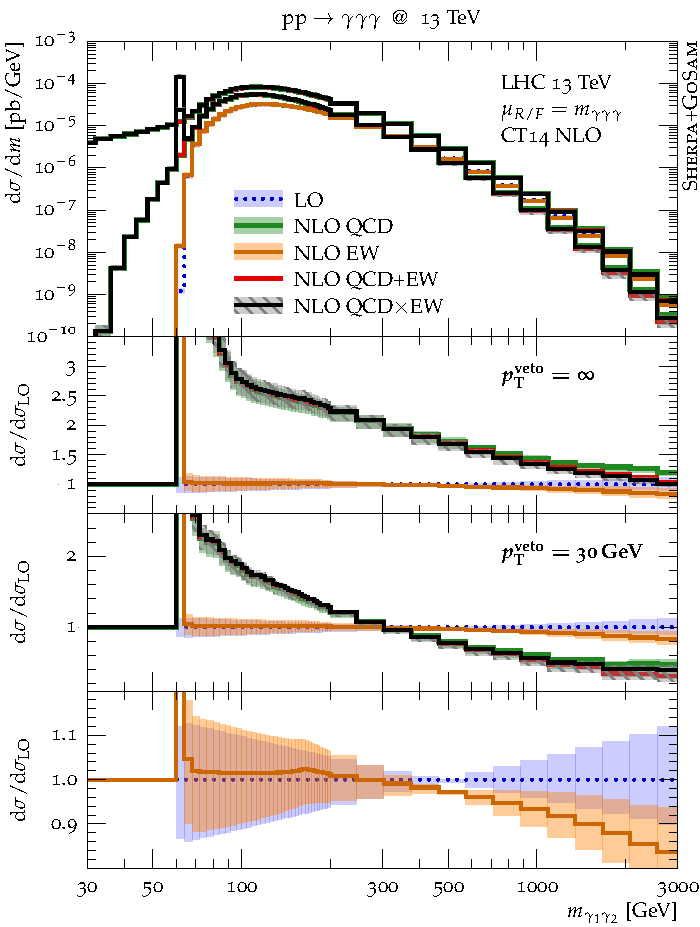
\includegraphics[width=0.32\textwidth]{figs_aaa/m_y1y2_comb_log}
  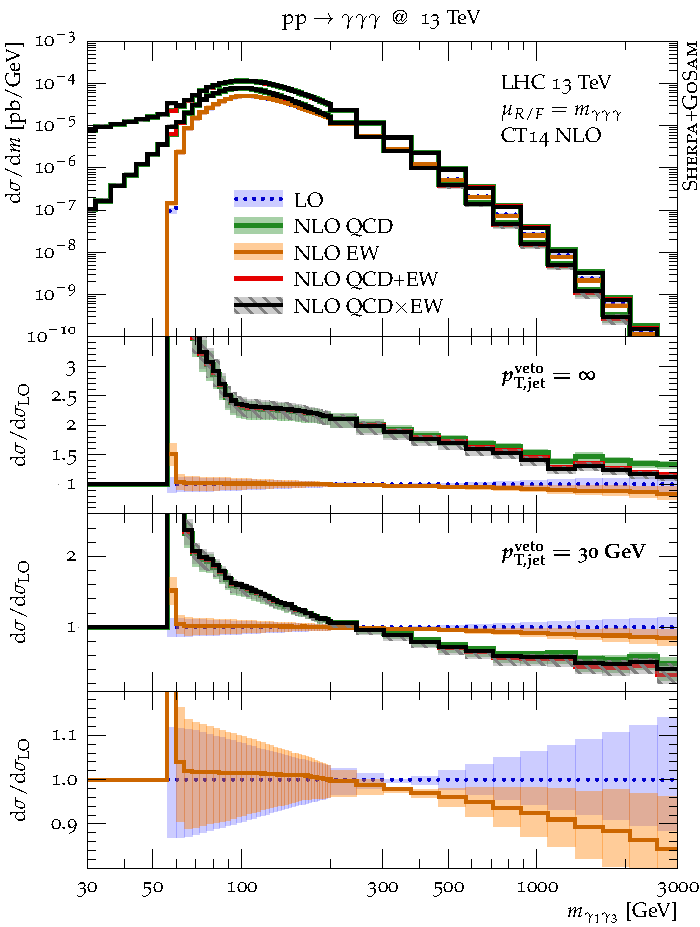
\includegraphics[width=0.32\textwidth]{figs_aaa/m_y1y3_comb_log}
  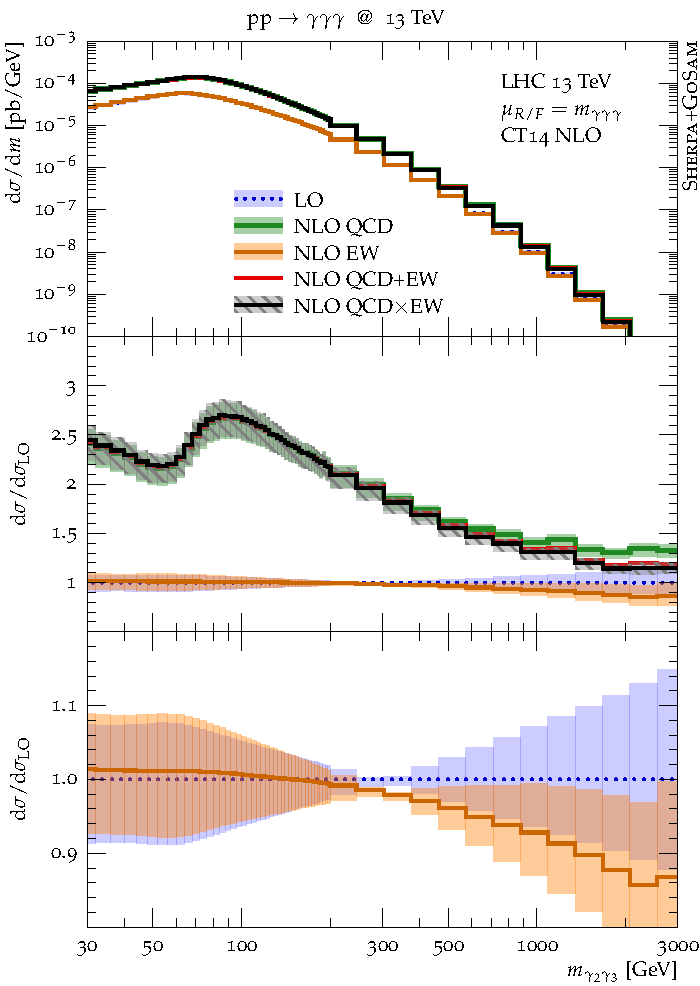
\includegraphics[width=0.32\textwidth]{figs_aaa/m_y2y3_comb_log}
  \caption{
    Pairwise invariant mass of the leading and subleading photon (left),
    leading and third leading photon (centre), subleading and third leading 
    photon (right) 
    in triple photon production at the LHC at 13\,TeV. 
    Details as in Fig.\ \ref{fig:aaa:pt}.\\
    \comment{MS: Spike in $m_{\gamma_1\gamma_2}$ is in NLO \QCDtEW\ 
             and comes from $\deltaEW\approx 10$ in this bin at the 
             edge of the LO phase space.}
    \label{fig:aaa:myy}
  }
\end{figure}

\begin{figure}[t!]
  \centering
  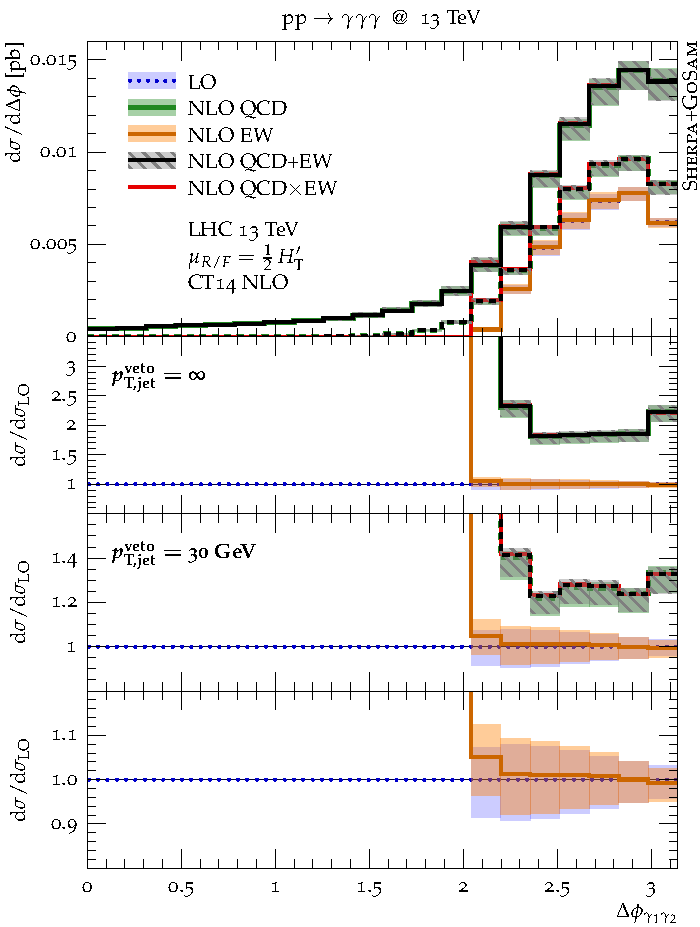
\includegraphics[width=0.32\textwidth]{figs_aaa/dphi_y1y2}
  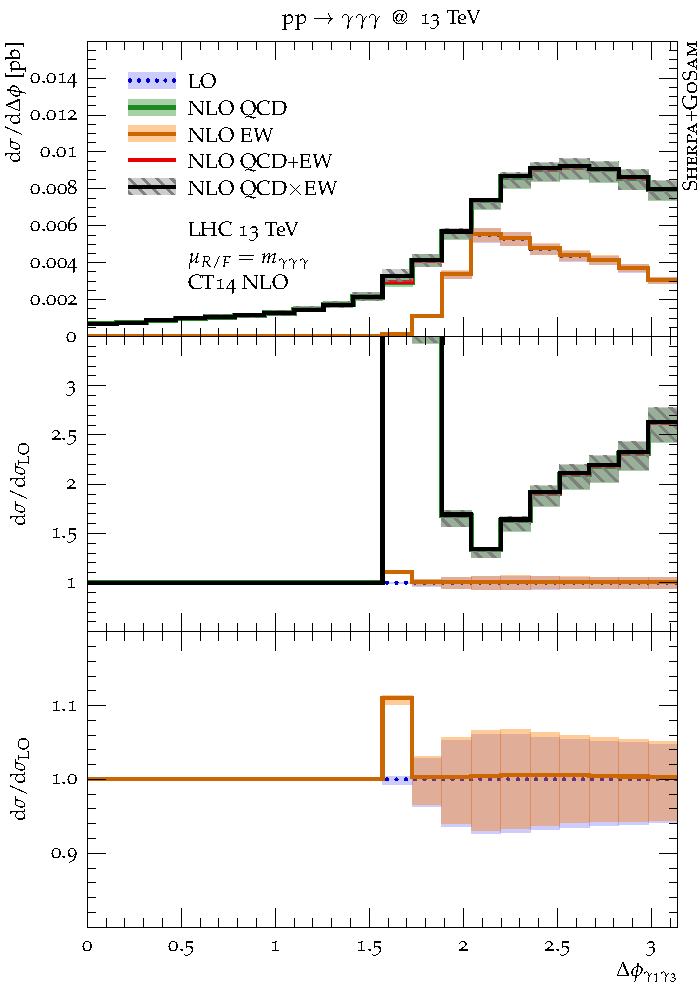
\includegraphics[width=0.32\textwidth]{figs_aaa/dphi_y1y3}
  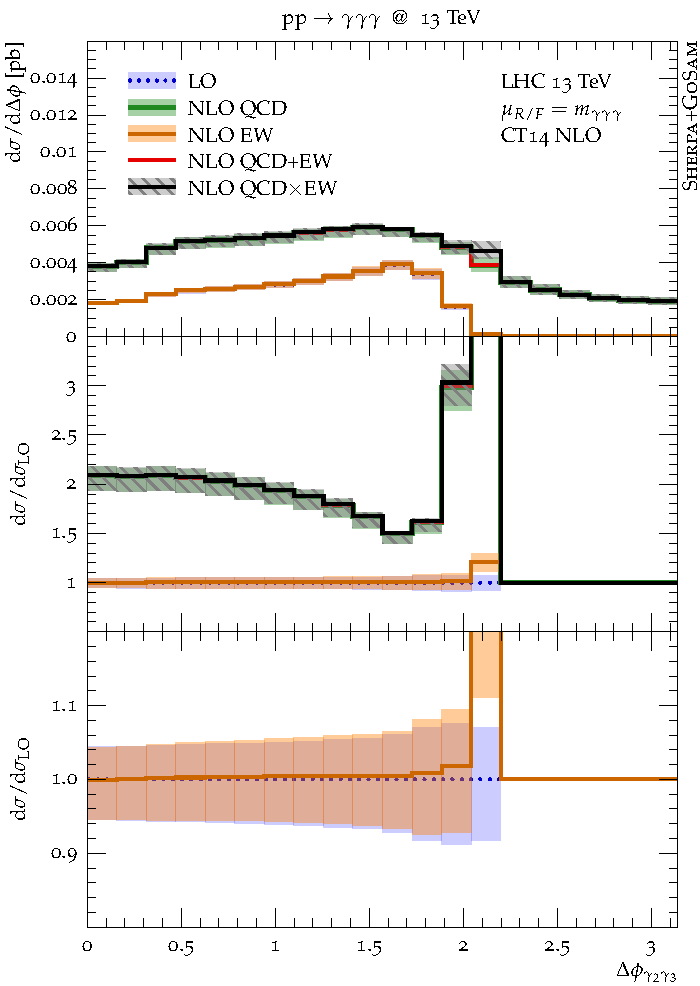
\includegraphics[width=0.32\textwidth]{figs_aaa/dphi_y2y3}
  \caption{
    Azimuthal separation of the leading and subleading photon (left),
    leading and third leading photon (centre), subleading and third leading 
    photon (right) 
    in triple photon production at the LHC at 13\,TeV. 
    Details as in Fig.\ \ref{fig:aaa:pt}.\\
    \comment{MS: Spike in $\Delta\phi_{\gamma_2\gamma_3}$ is in NLO \QCDtEW\ 
             and comes from $\deltaEW\approx 2$ in this bin at the 
             edge of the LO phase space.}
    \label{fig:aaa:dphi}
  }
\end{figure}

\begin{itemize}
  \item \pT of 3rd photon much softer than 1st and 2nd
  \item EW corrections to \pT of 1st and 2nd photon nearly identical and 
        $\approx -10\%$ at 500\,GeV, 3rd photon almost twice that.
  \item in all cases NLO EW outside LO uncertainty band
  \item NLO QCD dominated by real corrections, i.e.\ additional 
        jet emissions
  \item intensified through opening of new $qg$ channels and large 
        gluon luminosity
  \item can be controlled in fixed-order calculations through jet veto, 
        needs proper multijet merging
  \item because at LO the leading jet needs to be in the opposite 
        hemisphere as the subleading and third leading jet, 
        $m_{\gamma_1\gamma_2}$ and $m_{\gamma_1\gamma_3}$ 
        exhibit kinematic edges at LO
  \item kinematic conditions relaxed at NLO (both QCD and EW, 
        but QCD dominating), large corrections around those edges, 
        leads to artifacts in multiplicative combination
  \item NLO QCD very similar for $m_{\gamma_1\gamma_2}$ and 
	$m_{\gamma_1\gamma_3}$, $m_{\gamma_2\gamma_3}$ with interesting 
	structure around 80-90\,GeV
  \item $m_{\gamma_1\gamma_2}$ again exhibits small excess at $2m_W$
  \item small positive EW corrections at small $m_{\gamma\gamma}$ 
  \item $\approx -10\%$ at 1\,TeV for all $m_{\gamma\gamma}$ 
  \item NLO EW very similar for all $m_{\gamma\gamma}$ 
\end{itemize}



\subsection{\texorpdfstring{$\boldsymbol{\gamma\gamma\ell\nu}$}{aalnu} production}
\label{sec:results:aaw}

\comment{MS: is that $\ell^+$ or $\ell^-$?}

\begin{figure}[t!]
  \centering
  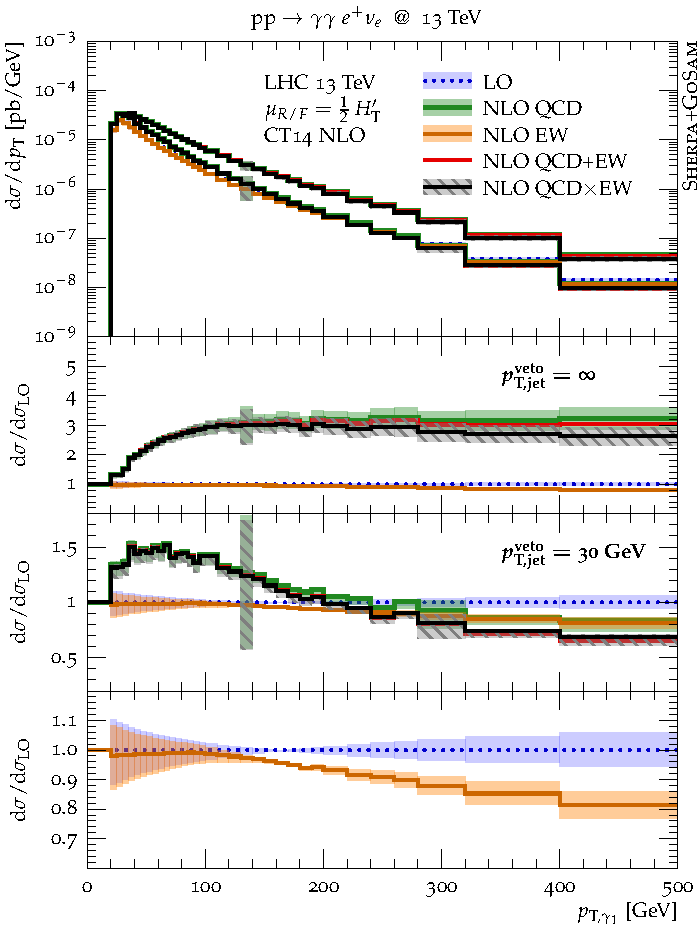
\includegraphics[width=0.32\textwidth]{figs_aaw/pT_y1}
  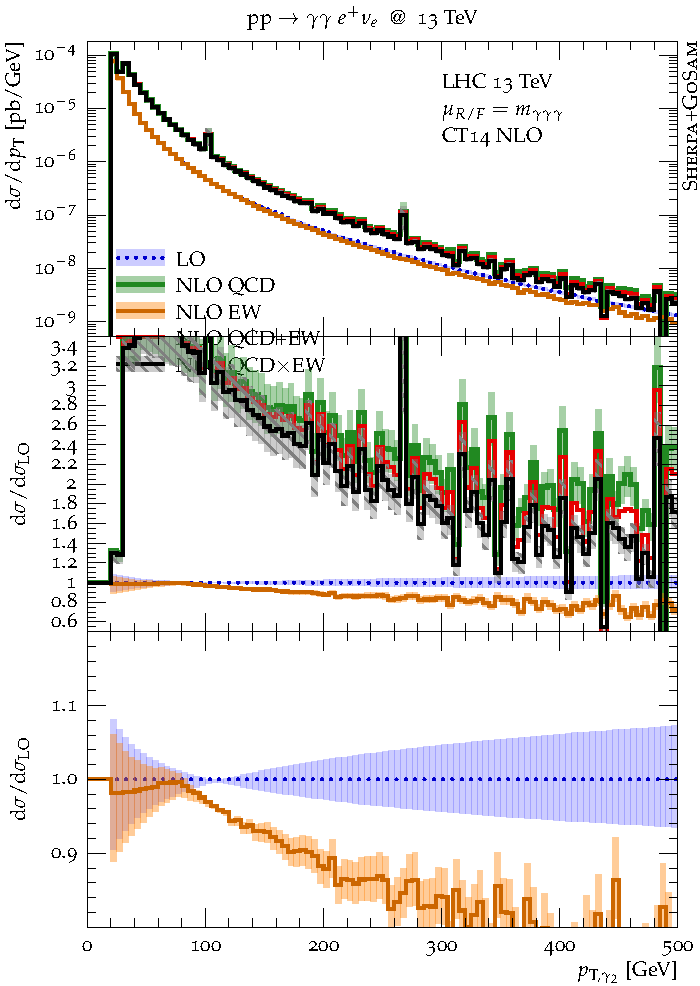
\includegraphics[width=0.32\textwidth]{figs_aaw/pT_y2}
  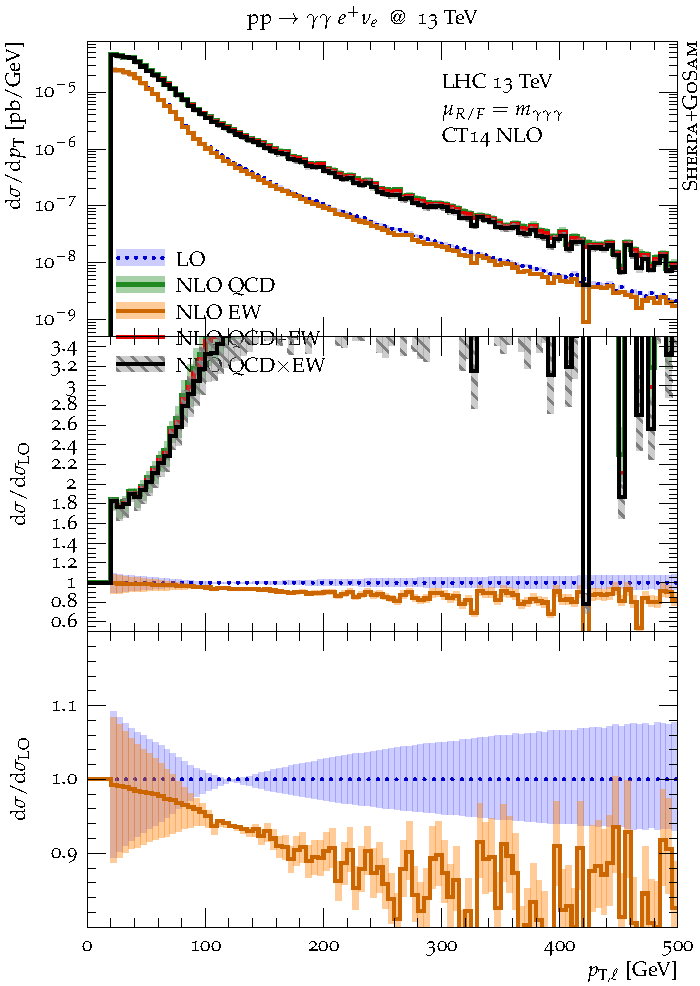
\includegraphics[width=0.32\textwidth]{figs_aaw/pT_l1}
  \caption{
    Transverse momentum of the leading (left), subleading (centre) 
    and third leading (right) photon at the LHC at 13\,TeV.
    \label{fig:aaw:pt}
  }
\end{figure}

\begin{figure}[t!]
  \centering
  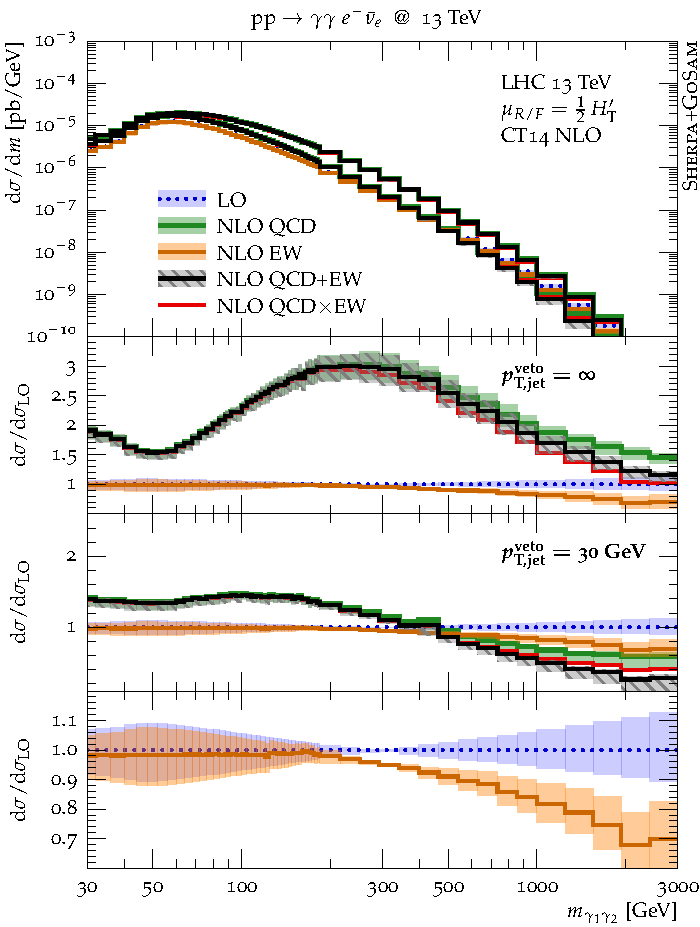
\includegraphics[width=0.32\textwidth]{figs_aaw/m_y1y2_comb_log}
  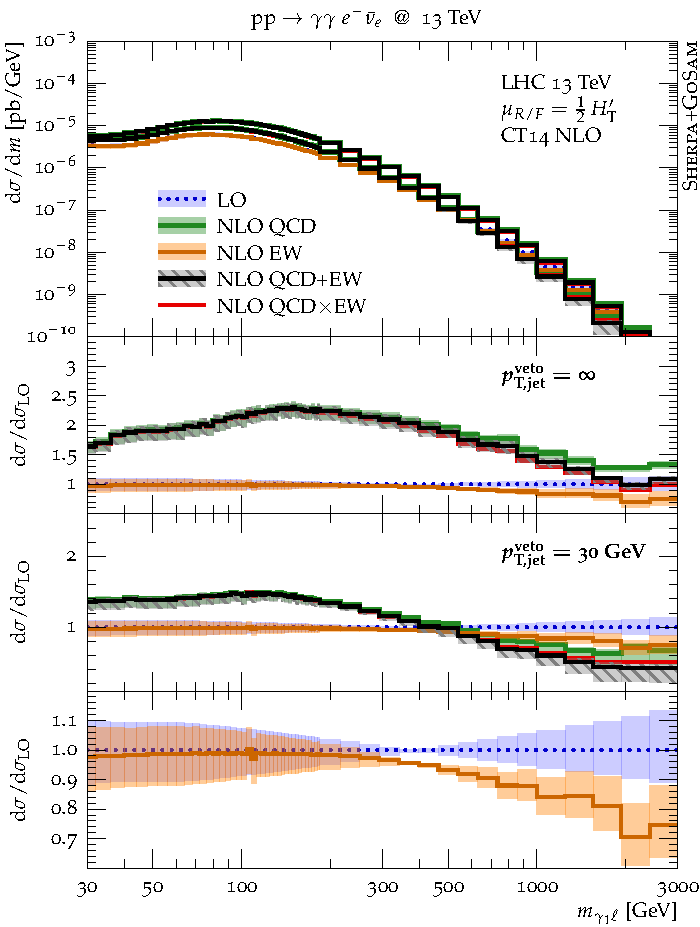
\includegraphics[width=0.32\textwidth]{figs_aaw/m_y1l1_comb_log}
  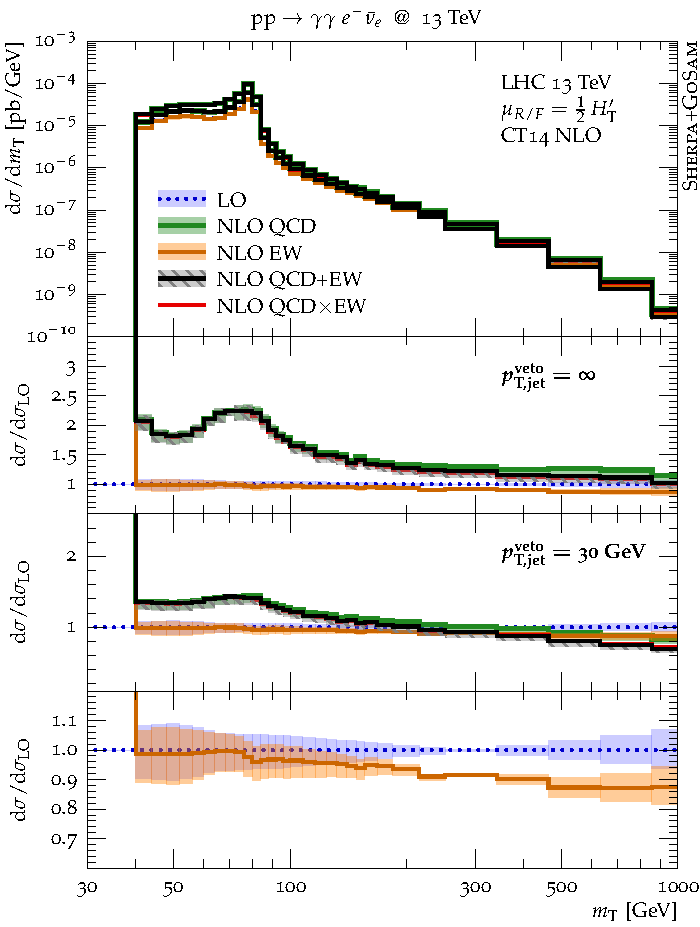
\includegraphics[width=0.32\textwidth]{figs_aaw/m_t_comb_log}
  \caption{
    Pairwise invariant mass of the leading and subleading photon (left),
    leading and third leading photon (centre), subleading and third leading 
    photon (right) at the LHC at 13\,TeV.\\
    \comment{MS: Spike in $m_{\gamma_1\gamma_2}$ is in NLO \QCDtEW 
             and comes from $\deltaEW\approx 10$ in this bin at the 
             edge of the LO phase space.}
    \label{fig:aaw:myy}
  }
\end{figure}

\begin{figure}[t!]
  \centering
  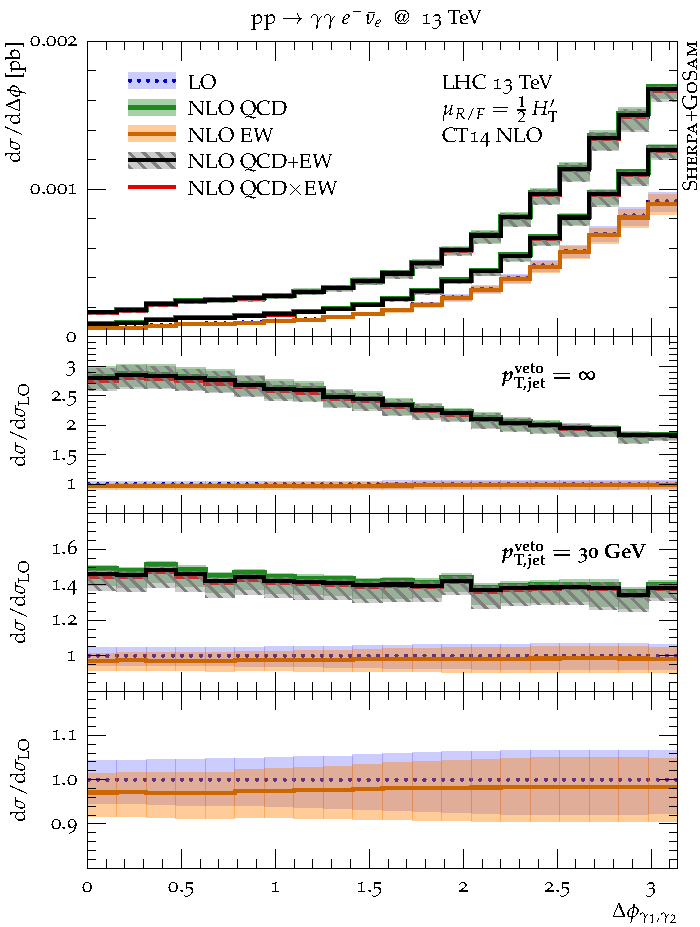
\includegraphics[width=0.32\textwidth]{figs_aaw/dphi_y1_y2}
  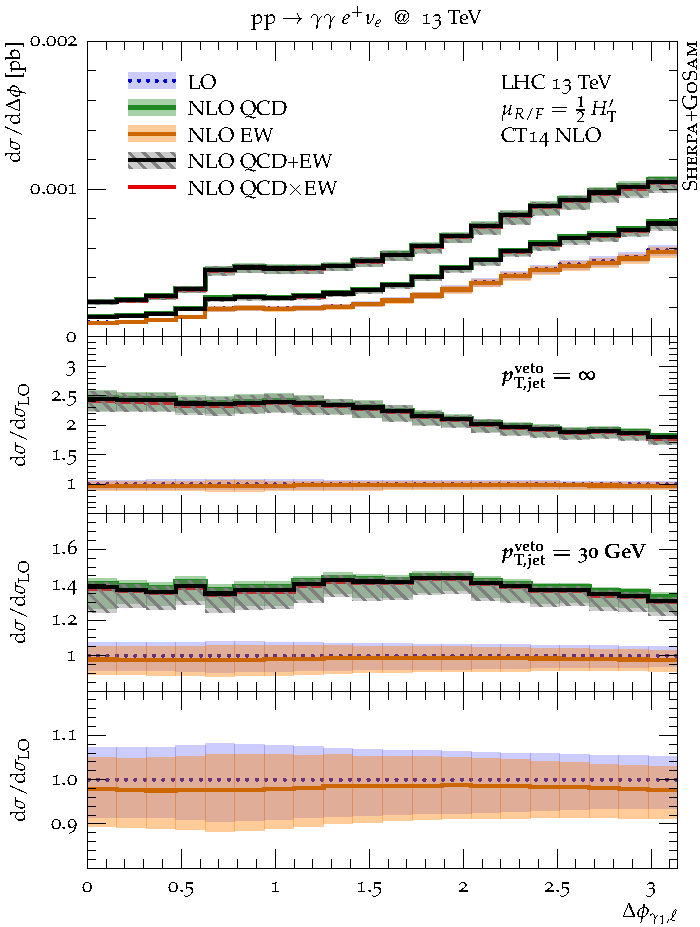
\includegraphics[width=0.32\textwidth]{figs_aaw/dphi_y1_l1}
  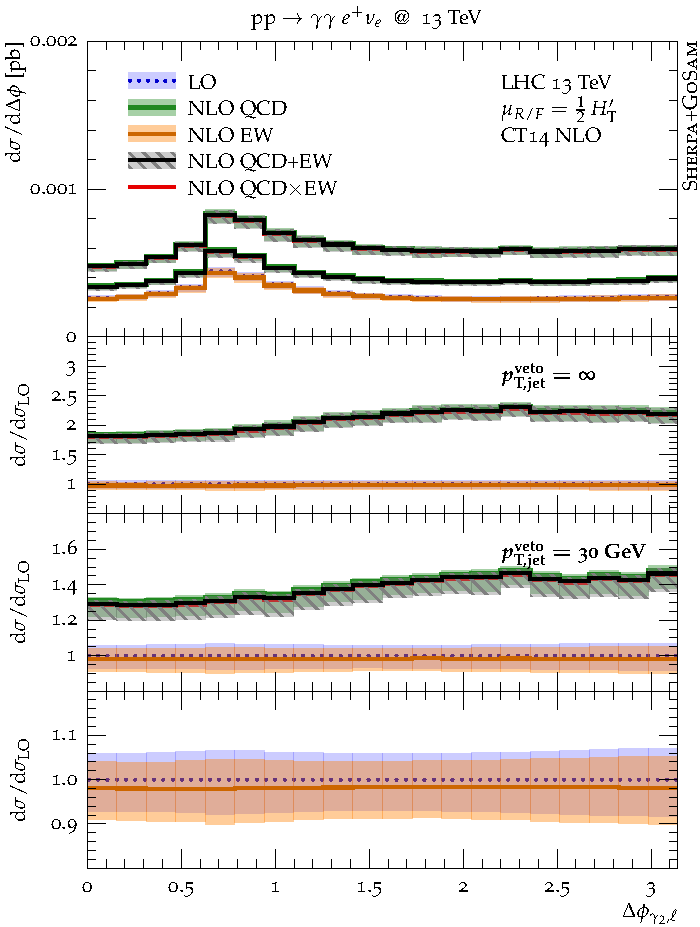
\includegraphics[width=0.32\textwidth]{figs_aaw/dphi_y2_l1}
  \caption{
    Azimuthal separation of the leading and subleading photon (left),
    leading and third leading photon (centre), subleading and third leading 
    photon (right) at the LHC at 13\,TeV.\\
    \comment{MS: Spike in $m_{\gamma_1\gamma_2}$ is in NLO \QCDtEW 
             and comes from $\deltaEW\approx 10$ in this bin at the 
             edge of the LO phase space.}
    \label{fig:aaw:dphi}
  }
\end{figure}


\subsection{\texorpdfstring{$\boldsymbol{\gamma\gamma\ell^+\ell^-}$}{aall} production}
\label{sec:results:aaz}

\begin{figure}[t!]
  \centering
  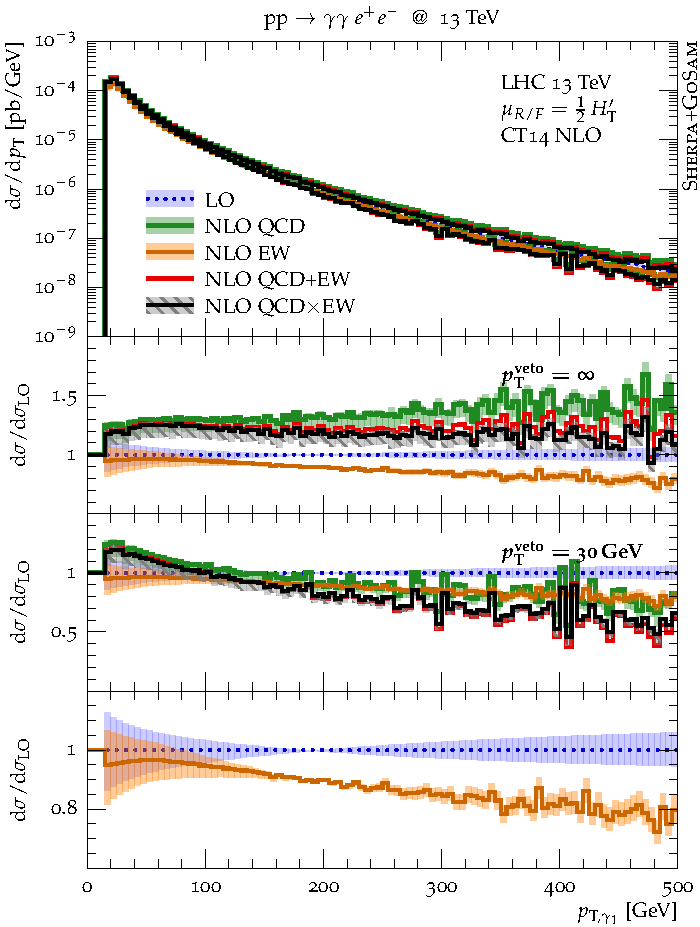
\includegraphics[width=0.32\textwidth]{figs_aaz/pT_y1}
  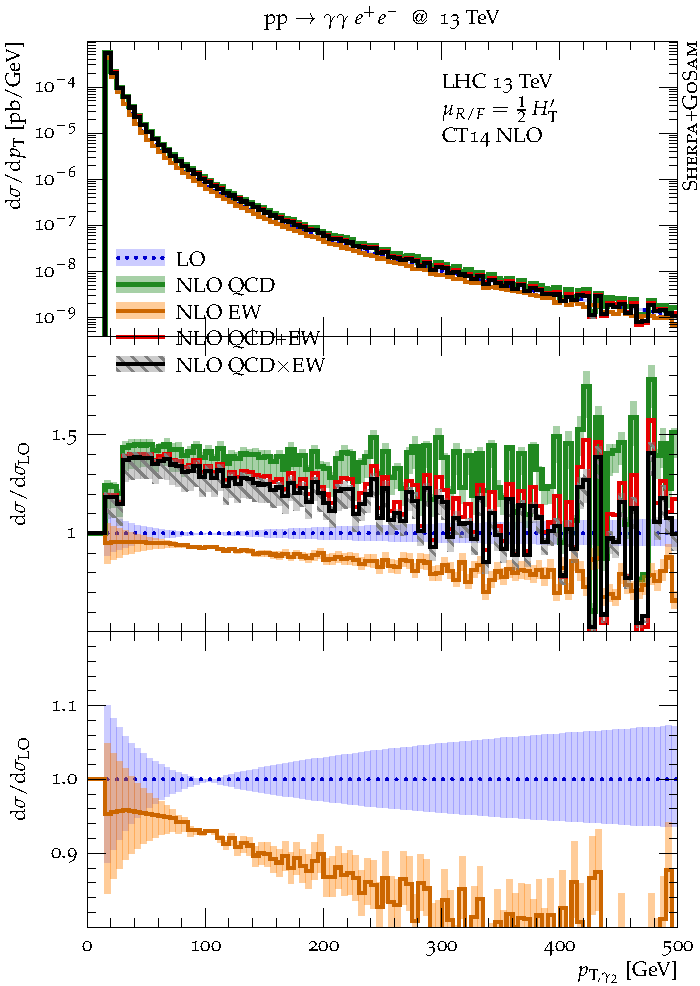
\includegraphics[width=0.32\textwidth]{figs_aaz/pT_y2}
  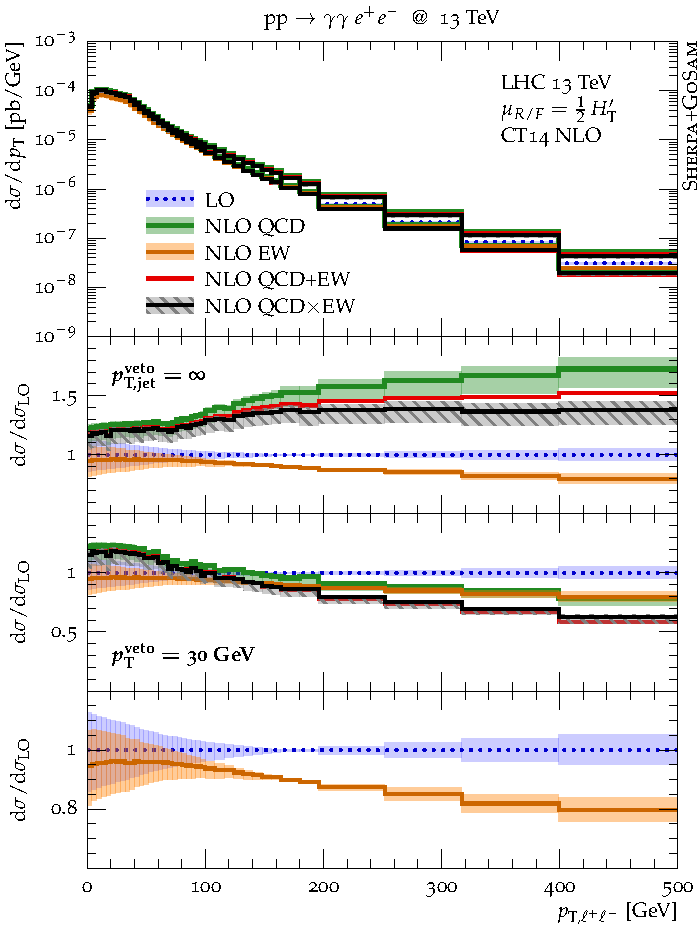
\includegraphics[width=0.32\textwidth]{figs_aaz/pT_l1l2_comb_log}
  \caption{
    Transverse momentum of the leading (left) and subleading (centre) 
    photon as well as the dressed lepton pair (right) 
    in diple photon production in association with a lepton pair 
    at the LHC at 13\,TeV. 
    Details as in Fig.\ \ref{fig:aaa:pt}.
    \label{fig:aaz:pt}
  }
\end{figure}

\begin{figure}[t!]
  \centering
  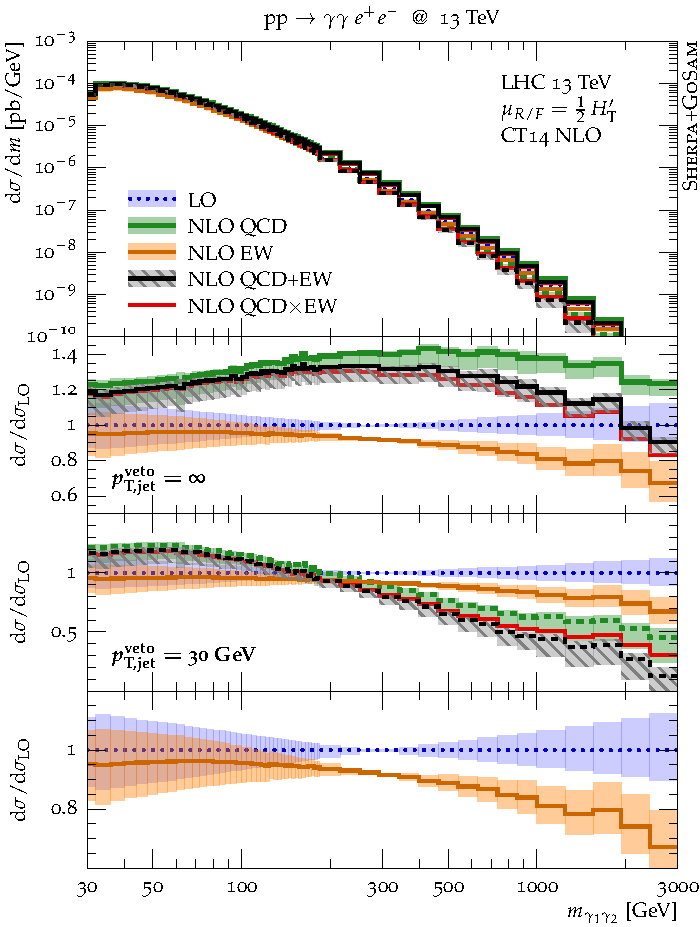
\includegraphics[width=0.32\textwidth]{figs_aaz/m_y1y2_comb_log}
  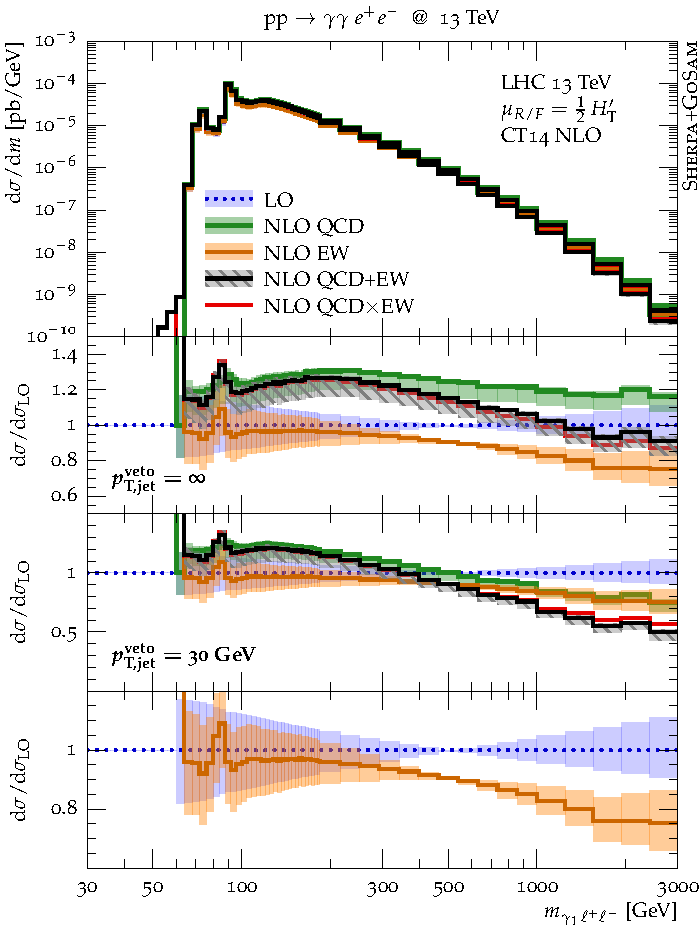
\includegraphics[width=0.32\textwidth]{figs_aaz/m_y1l1l2_comb_log}
  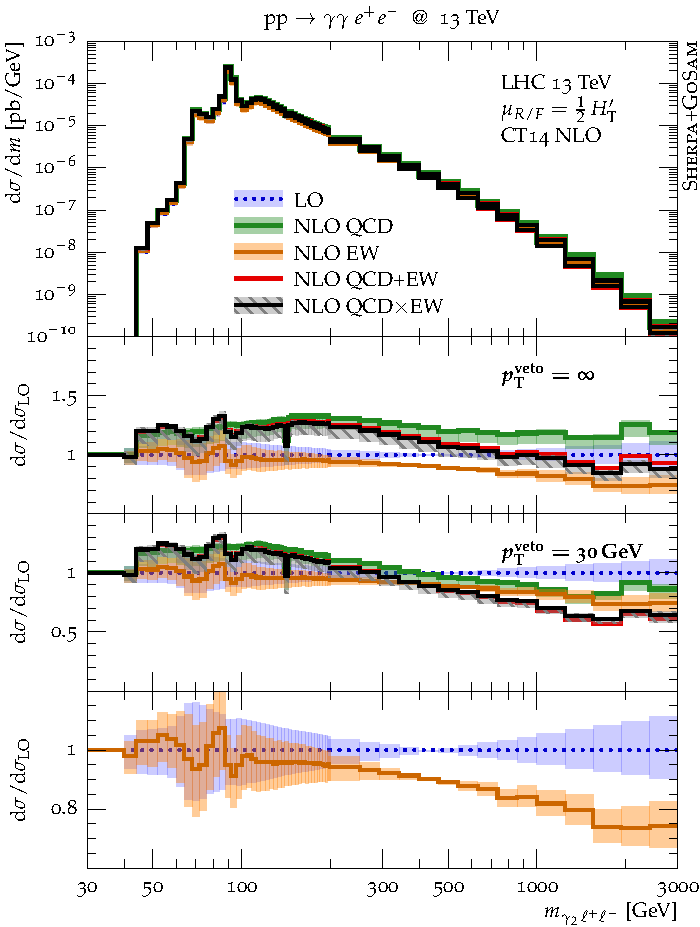
\includegraphics[width=0.32\textwidth]{figs_aaz/m_y2l1l2_comb_log}
  \caption{
    Pairwise invariant mass of the leading and subleading photon (left),
    the leading photon and the lepton pair (centre), and the subleading 
    photon and the lepton pair (right)
    in diple photon production in association with a lepton pair 
    at the LHC at 13\,TeV. 
    Details as in Fig.\ \ref{fig:aaa:pt}.\\
    \comment{MS: Spike in $m_{\gamma_1\ell_1\ell_2}$ is in NLO \QCDtEW\ 
             and comes from $\deltaEW\approx 10$ in this bin at the 
             edge of the LO phase space.}
    \label{fig:aaz:myy}
  }
\end{figure}

\begin{figure}[t!]
  \centering
  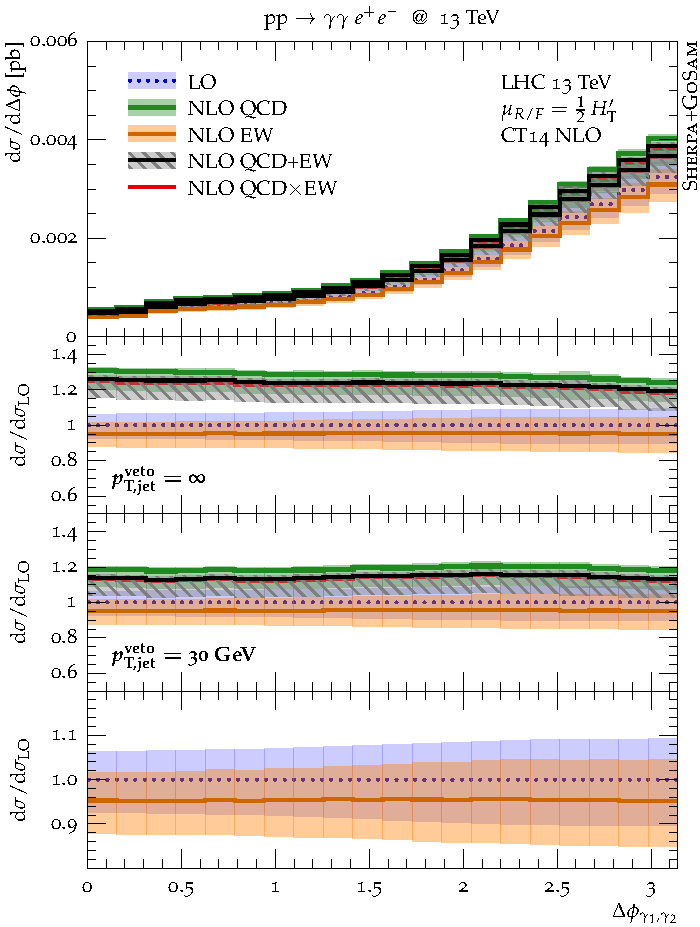
\includegraphics[width=0.32\textwidth]{figs_aaz/dphi_y1_y2}
  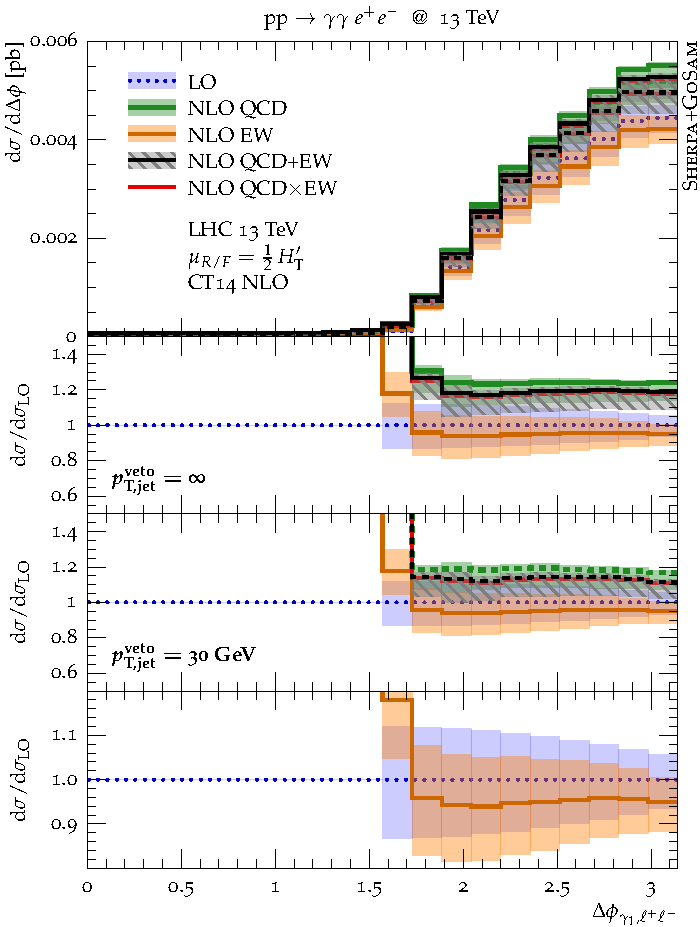
\includegraphics[width=0.32\textwidth]{figs_aaz/dphi_y1_l1l2}
  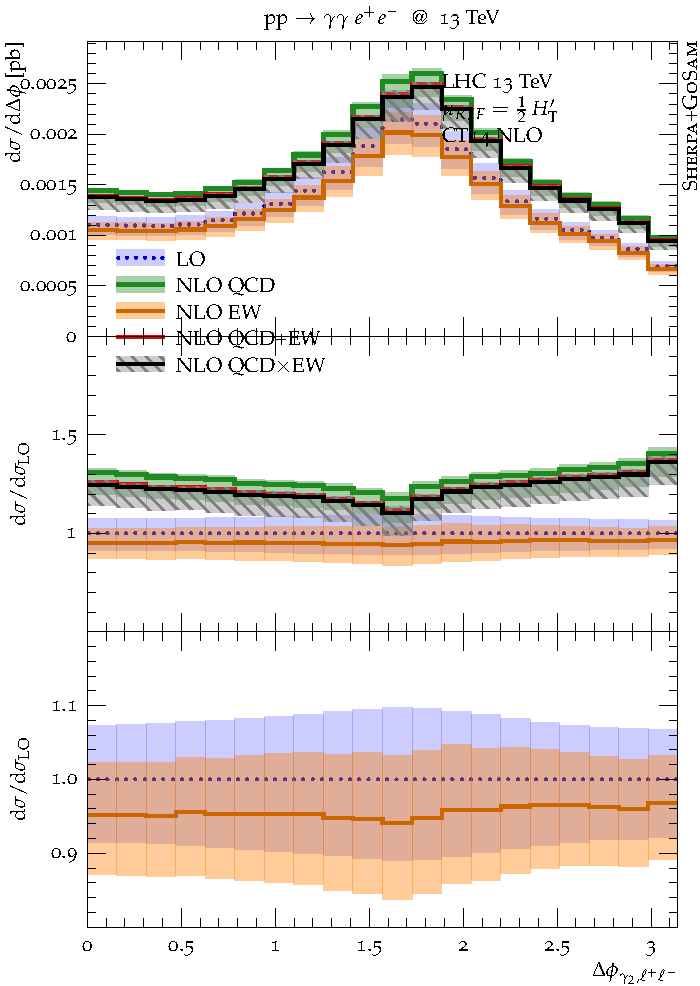
\includegraphics[width=0.32\textwidth]{figs_aaz/dphi_y2_l1l2}
  \caption{
    Azimuthal separation of the leading and subleading photon (left),
    the leading photon and the lepton pair (centre), and the subleading 
    photon and the lepton pair (right)
    in diple photon production in association with a lepton pair 
    at the LHC at 13\,TeV. 
    Details as in Fig.\ \ref{fig:aaa:pt}.\\
    \comment{MS: Spike in $\Delta\phi_{\gamma_1,\ell_1\ell_2}$ is in NLO \QCDtEW\ 
             and comes from $\deltaEW\approx 10$ in this bin at the 
             edge of the LO phase space.}
    \label{fig:aaz:dphi}
  }
\end{figure}



